\chapter{GE1/1 measured parameters} % (fold)
\label{cha:ge1_1_measured_parameters}
In lab at CERN several parameters of the tested GE1/1 detectors are measured.
They are - electric field, voltage across each GEM foil, gain and rate for both GE1/1, i.e., GE11\_IV and GE11\_IV\_GIF.
% They are electric field, voltage across each GEM foil. Also, the gain and rate for both GE1/1, i.e., GE11\_IV and GE11\_IV\_GIF, are measured.

The high voltage configuration used during the beam test is shown in Fig.~\ref{fig:HV_configuration}. 
\begin{figure}[htbp]
    \centering
    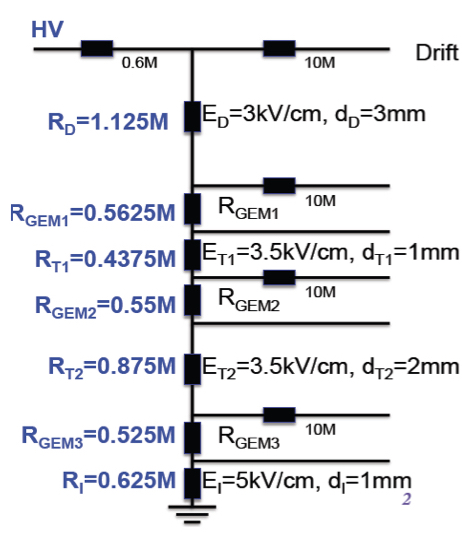
\includegraphics[width=0.40\textwidth]{figures/GEM/HV_divider_gem_testbeam_2014.jpeg}
    \caption{High voltage divider configuration as used in the 2014 beam test campaign.}
    \label{fig:HV_configuration}
\end{figure}


Also, the voltage across the GEM foils and  the electric field  with respect to the current in the voltage divider is shown in Fig.~\ref{fig:GEM_voltage_electricfield}. 
\begin{figure}[htbp]
    \centering
    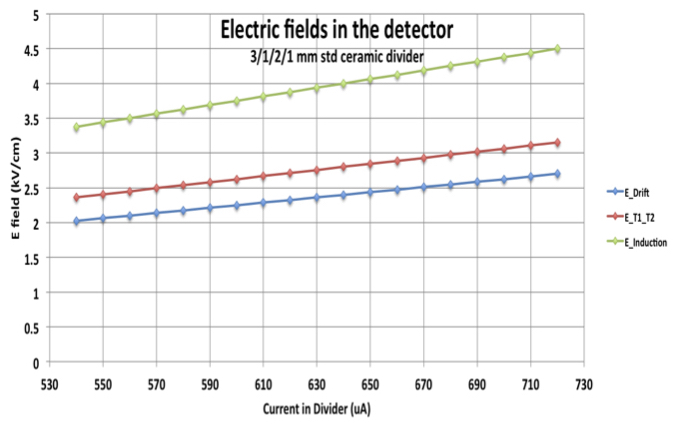
\includegraphics[width=0.5\textwidth]{figures/GEM/GE11_IV_ElectricField_detector.jpeg}%
    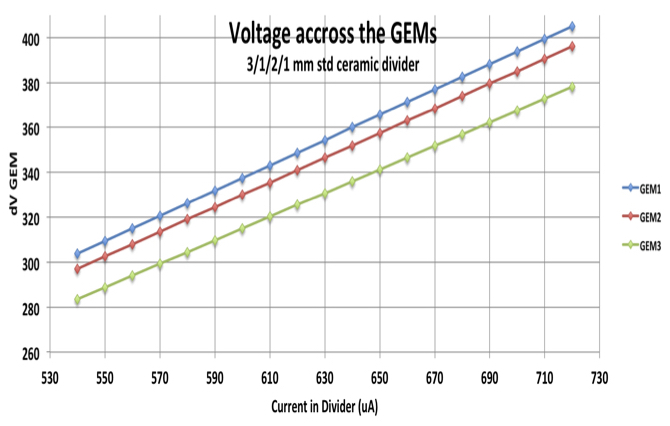
\includegraphics[width=0.5\textwidth]{figures/GEM/GE11_IV_VoltageAcross_GEM.jpeg}
    \caption{Electric field (left) and voltage across each GEM foil (right) for the tested GE1/1 detector.}
    \label{fig:GEM_voltage_electricfield}
\end{figure}


The gain of the detector was measured in the lab using an X-ray source for both $Ar:CO_2$ and $Ar:CO_2:CF_4$ gas mixture and is shown in Fig.~\ref{fig:gain_GE1/1_IV_GIF} and ~\ref{fig:gain_GE1/1_IV}.
\begin{figure}[htbp]
    \centering
    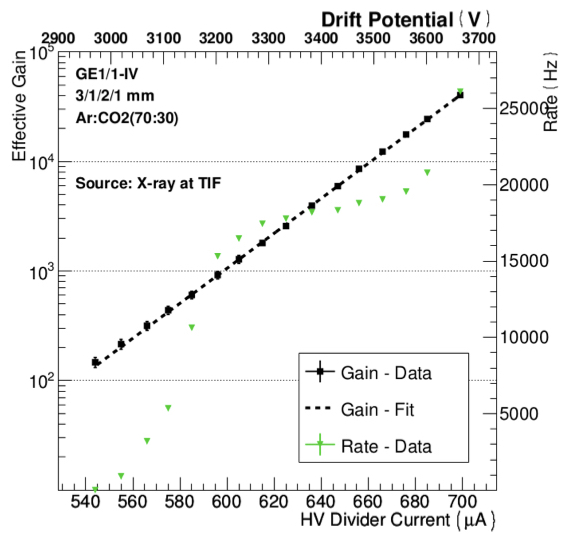
\includegraphics[width=0.5\textwidth]{figures/GEM/Gain_curve_GE11_IV_Ar_CO2.jpeg}%
    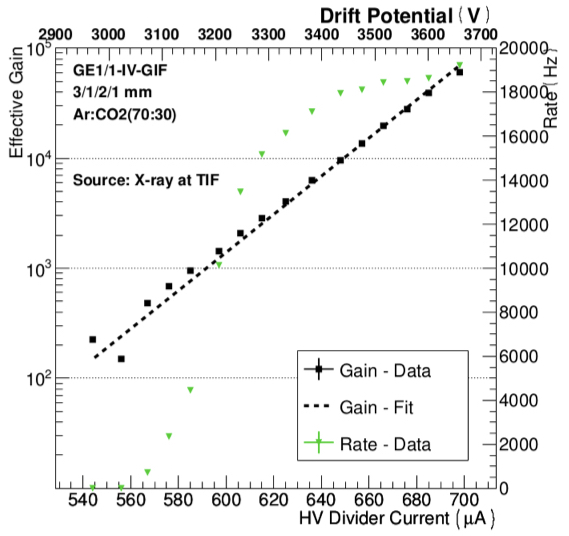
\includegraphics[width=0.5\textwidth]{figures/GEM/Gain_curve_GE11_IV_GIF_Ar_CO2.jpeg}
    \caption{Gain and rate variation for $Ar:CO_2$ (70:30) with respect to the current supplied to the high voltage divider for GE1/1-IV (left) and GE1/1-IV-GIF (right).}
    \label{fig:gain_GE1/1_IV}
\end{figure}
\begin{figure}[htbp]
    \centering
    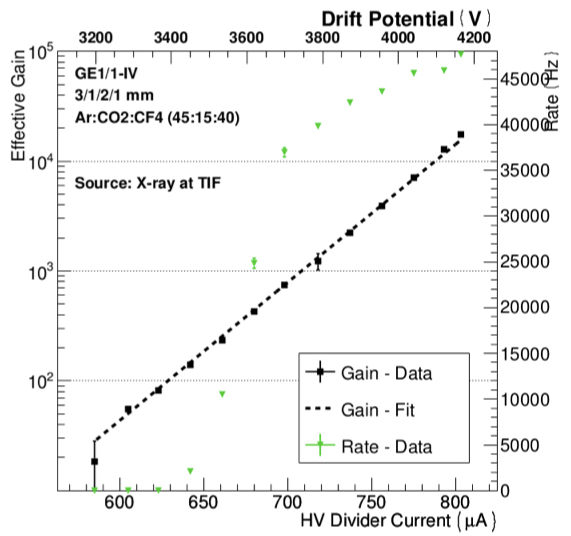
\includegraphics[width=0.5\textwidth]{figures/GEM/Gain_curve_GE11_IV_Ar_CO2_CF4.jpeg}%
    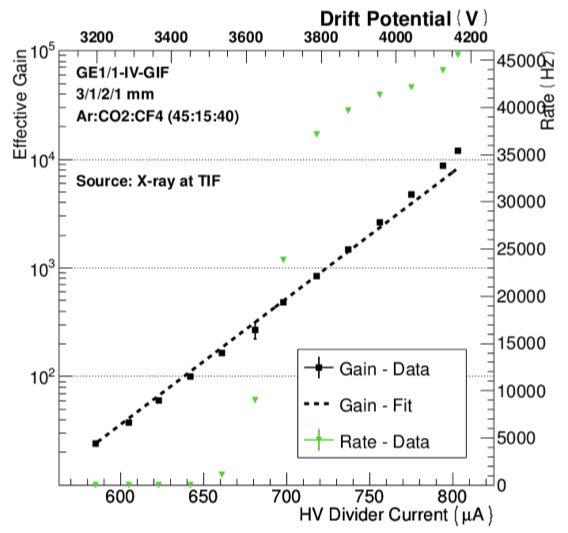
\includegraphics[width=0.5\textwidth]{figures/GEM/Gain_curve_GE11_IV_GIF_Ar_CO2_CF4.jpeg}
    \caption{Gain and rate variation for $Ar:CO_2:CF_4$ (45:15:40) with respect to the current supplied to the high voltage divider for GE1/1-IV (left) and GE1/1-IV-GIF (right).}
    \label{fig:gain_GE1/1_IV_GIF}
\end{figure}




% subsubsection _information_of_gem_detectors_used_in_test_beam (end)

% chapter ge1_1_measured_parameters (end)